\documentclass[10pt]{article}
\usepackage[utf8]{inputenc}
\usepackage[T1]{fontenc}
\usepackage{lmodern}
\usepackage{geometry}
\usepackage{graphicx}
\usepackage{float}
\usepackage{upquote}
\usepackage{setspace}
\usepackage{tabularx}
\usepackage{amsmath, amssymb}
\usepackage{siunitx}
\usepackage{circuitikz}
\usepackage{tikz}
\usepackage{physics}
\geometry{a4paper, left=20mm, right=20mm, top=20mm, bottom=20mm}
\usetikzlibrary{angles, quotes}
\tikzset{>=latex}
\definecolor{amber}{rgb}{1.0, 0.5, 0}
\definecolor{darkmagenta}{rgb}{0.55, 0.0, 0.55}
\setlength{\parindent}{0pt}
\setlength{\parskip}{1em}
%\usepackage{fancyhdr}
%\pagestyle{fancy}
%\fancyhf{}
%\fancyhead[C]{Electricity & Electromagnetism}
%\fancyfoot[C]{\thepage}
%\renewcommand{\headrulewidth}{0pt}
%\renewcommand{\footrulewidth}{0pt}

%%%%%%%%%%%%%%%%%%%%%%%%%%%%%%%%%%%%%%%%%%%%%%%%%%%%%%%%%%%%%%%%%%%%%%%%%%%%%
\begin{document}
\title{Influence of Magnetic Fields on Direct and Alternating Currents - I}
\date{\vfill
\today}
\author{Lucas Helal}
\maketitle
\newpage
\tableofcontents
\newpage
	\section{Introduction}
	Here I discuss the impact of a magnetic field in direct current (DC) and
	alternating current (AC) when generated by a third electrical conductor - i.e.,
	under the influence of external electromagnetic field generated by a body
	acting as an inductor. This involves the \emph{Biot-Savart Law}, \emph{Faraday's
	Law}, \emph{Lenz and Faraday-Lenz Laws}, \emph{Ohm's Laws} and \emph{Gauss' Laws}
	and \emph{Maxwell's Laws} mainly, among others. It also takes into account: to
	consider voltage level, type of current, signal type, operating frequency, electric
	field magnitude, and the type of electric field.

	For the sake of simplicity but maintaining formalism, I am identifying the variables
	as follows:
	\begin{itemize}
		\item {$\vec{B}$: Magnetic field;}

		\item {$\mu_{0}$: Magnetic permeability of free space;}

		\item {$I$: Current;}

		\item {$d\vec{l}$: Differential length element of the wire;}

		\item {$\vec{r}$: Position vector from the wire element to the point where the magnetic field is being calculated;}

		\item {$\vec{r}_{p}$: Position vector of the point to be determined in the field;}

		\item {$\vec{r}_{l}$: Position vector that goes from the origin to a point on the wire;}

		\item {$L$: Length of the wire;}

		\item {$\varepsilon$: Electromotive force;}

		\item {$\Phi_{B}$: Magnetic flux;}

		\item {$Q_{\text{enc}}$: Charge enclosed by the surface;}

		\item {$\varepsilon_{0}$: Vacuum permittivity;}

		\item {$V$: Voltage;}

		\item {$R$: Resistance;}

		\item {$f$: Frequency;}

		\item {$t$: Time;}

		\item {$\theta$: Angle.}

		\item {$\hat{\mathbf{r}}$: Unit vector from the current element to the point where the field is calculated.}

		\item {$r$: Distance between the current element and the point.}

		\item {$\mathbf{E}$: Electric field.}

		\item {$d\mathbf{A}$: Differential area element.}

		\item {$Q$: Electric charge.}

		\item {$\sin$: Sine function.}

		\item {$\cos$: Cosine function.}

		\item {$\tan$: Tangent function.}

		\item {$\pi$: Pi constant as $\approx \ 3.14159265358979323846 \dots$.}
	\end{itemize}

	\section{Basic Concepts}
	\subsection{Direct Current - DC}
	Direct current is the unidirectional flow of electric charge. It is
	represented by the equation: $I_{DC}= \frac{dQ}{dt}$ where $I_{DC}$ is the direct
	current, $Q$ is the electric charge, and $t$ is the time.

	\subsection{Alternating Current - AC}
	Alternating current is the flow of electric charge that periodically reverses direction.
	It is represented by the equation: $I_{AC}= I_{max}\sin(2\pi f t)$ where $I_{AC}$
	is the alternating current, $I_{max}$ is the maximum current, $f$ is the frequency,
	and $t$ is the time.

	\section{Influence of Electromagnetic Fields}

	Let's start with an example of the Hall effect, in which the electrical
	current can be influenced by a magnetic field.

	The full form of the Hall Effect equation is given by:

	\begin{equation}
		V_{H} = \frac{IB}{ne},
	\end{equation}

	where $V_{H}$ is the Hall voltage, $I$ is the current, $B$ is the magnetic field,
	$n$ is the charge carrier density, and $e$ is the elementary charge.

	Below, in Python code, I simulated the effect of a magnetic field $\vec{B}$ on
	a current $I$ in a conductor with charge carrier density $n$ and elementary charge
	$e$ as constants. I also considered the voltages of either 220V of 127V, and the
	resistance of the conductor as $R = R \ \Omega$.
{
  \centering
	\includegraphics*[width=0.6\textwidth]{
		/Users/lucashelal/Desktop/eel/eletromag/plots/magnetic_field_1.png
	}
}
{
\begin{verbatim*}
  import pandas as pd
  import seaborn as sns
  import matplotlib.pyplot as plt

  # load seaborn
  sns.set_theme()

  # constants definition

  d = 0.001 # cable width in meters
  R_H = 1e-3 # Hall coefficient in m^3/C

  # magnetic field space 
  B = np.linspace(0.01, 1, 1000) # 0.01 T to 1 T

  # voltages

  V_220 = 220
  V_127 = 127

  # lets assume that V_H is proportional to V - add a factor
  k = 0.1
  V_H_220 = k * V_220
  V_H_127 = k * V_127

  # current as function of B for either 220 or 127 V
  I_220 = (V_H_220 * d) / (R_H * B)
  I_127 = (V_H_127 * d) / (R_H * B)

  # create a dataframe

  data = np.column_stack((B, I_220, I_127))
  data = pd.DataFrame(data, columns=['B', 'I_220', 'I_127'])
  data_melted = pd.melt(data, id_vars='B', value_vars=['I_220', 'I_127'], var_name='Voltage', value_name='Current')

  # plot
  plt.figure(figsize=(10, 6))
  sns.lineplot(x='B',y='Current', hue='Voltage', data=data_melted)
  plt.title('Current as function of magnetic field for different voltages')
  plt.grid(True)
  plt.show()
\end{verbatim*}



	\newpage

	The Biot-Savart Law describes the magnetic field generated by an electric
	current. It is given by:
	\[
		\mathbf{B}= \frac{\mu_{0}}{4\pi}\int \frac{I d\mathbf{l} \times \hat{\mathbf{r}}}{r^{2}}
	\]
	where $\mathbf{B}$ is the magnetic field, $\mu_{0}$ is the vacuum permeability,
	$I$ is the current, $d\mathbf{l}$ is the element of length through which the current
	flows, $\hat{\mathbf{r}}$ is the unit vector from the current element to the
	point where the field is calculated, and $r$ is the distance between the current
	element and the point.
	\subsection{Faraday-Lenz's Law}
	Faraday-Lenz's Law states that the induced electromotive force (EMF) in any
	closed circuit is equal to the negative of the time rate of change of the
	magnetic flux through the circuit:
	\[
		\varepsilon = -\frac{d\Phi_{B}}{dt}
	\]
	where $\varepsilon$ is the EMF and $\Phi_{B}$ is the magnetic flux.

	\subsection{Gauss's Law}
	Gauss's Law relates the distribution of electric charge to the resulting electric
	field:
	\[
		\oint \mathbf{E}\cdot d\mathbf{A}= \frac{Q_{\text{enc}}}{\varepsilon_{0}}
	\]
	where $\mathbf{E}$ is the electric field, $d\mathbf{A}$ is the differential area
	element, $Q_{\text{enc}}$ is the charge enclosed by the surface, and $\varepsilon
	_{0}$ is the vacuum permittivity.

	\subsection{Ohm's Law}
	Ohm's Law states the relationship between voltage, current, and resistance in an
	electrical circuit:
	\[
		V = IR
	\]
	where $V$ is the voltage, $I$ is the current, and $R$ is the resistance.

	\subsection{Tesla's Postulates}
	Nikola Tesla's contributions to the understanding of electromagnetic fields
	and alternating current systems are numerous. One of his fundamental postulates
	emphasizes the efficiency and necessity of alternating current for long-distance
	electrical power transmission.

	\newpage

	\section{The Biot-Savart Law}

	The \emph{Biot-Savart Law} mathematically describes magnetic field generated
	by a current-carrying wire, allowing us to calculate the magnetic field at any
	point in space. The Law is fundamental to the study of magnetism and
	electromagnetism, and it is used to calculate the magnetic field produced by various
	current distributions, such as straight wires, loops, and solenoids, \emph{a
	cornerstorne in the power generation, transmission and distribution systems to
	all end-users. The Law is also used in the design of electric motors, transformers,
	and inductors and in the study of magnetic materials.}

	Some of the applications of the \emph{Biot-Savart Law} include:
	\begin{itemize}
		\item Calculation of the magnetic field produced by a current-carrying wire.

		\item Calculation of the magnetic field produced by a current loop.

		\item Calculation of the magnetic field produced by a solenoid.

		\item Calculation of the magnetic field produced by a toroid.

		\item Calculation of the magnetic field produced by a straight wire.

		\item Calculation of the magnetic field produced by a circular arc.

		\item Calculation of the magnetic field produced by a current sheet.

		\item Calculation of the magnetic field produced by a finite wire.

		\item Calculation of the magnetic field produced by a semi-infinite wire.

		\item Calculation of the magnetic field produced by a coaxial cable.
	\end{itemize}

	The canonical form of the \emph{Biot-Savart Law} is given by:

	\begin{equation}
		\vec{B}= \frac{\mu_{0} I}{4\pi}\int \frac{d \vec{l} \times \vec{r}}{|\vec{r}|^{2}}
	\end{equation}

	where $\vec{B}$ is the magnetic field, $\mu_{0}$ is the magnetic permeability of
	free space, $I$ is the current, $d \vec{l}$ is the differential length element
	of the wire, $\vec{r}$ is the position vector that goes from the wire element
	to the point where the magnetic field is being calculated, and $|\vec{r}|$ is the
	magnitude of the position vector.

	Below there is a plot of a current-carrying wire, where the magnetic field is
	calculated at a point $P$. This, together with Faraday's Law, is the basis for
	the operation of electric generators; the Lenz's Law, which is the basis for the
	operation of electric motors; and the Ampère's Law, which is the basis for the
	operation of transformers and Tesla's discoveries on the generation of high-voltage
	currents gives us the basis for the operation of the power transmission and distribution
	systems, and also the alternating current (AC) systems. Below there is a plot of
	a direct-current (DC) system versus an alternating-current (AC) system given the
	presence and influence of a magnetic field induced by a current-carrying wire.

	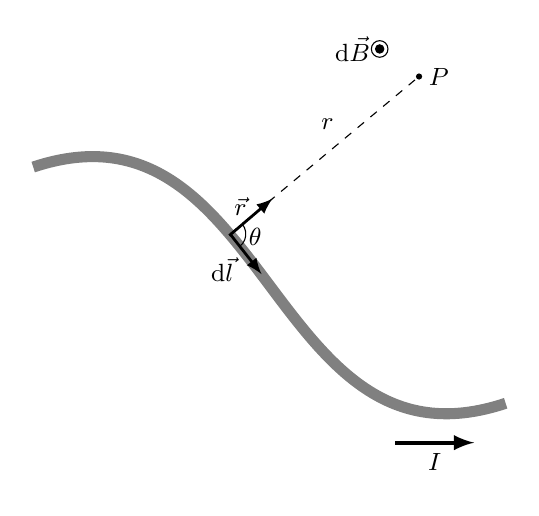
\begin{tikzpicture}[scale=1]
	% Grid
%	\draw[help lines] (0,0) grid (8,8);
	
	% Current Cable	
	\draw[line width=4, color = gray] (1,4) ..controls (4,5) and (4,0).. (7,1) ;
	
	% Vectors
	\draw[dashed] (3.5,3.15)coordinate(B) -- +(2.4,2) node [pos=0.6, above left] {\small$r$};
	\draw[line width = 1,->] (3.5,3.15) -- +(0.4,-0.51)coordinate(A) ;
	\draw[line width = 1,->] (3.49,3.13) -- (4.04,3.6)coordinate(C) node [pos = 0.26, above, black] {\small$\vec{r}$} ;

	
	% Point
	\filldraw (5.9, 5.15) circle (0.9pt) node [right] {\small$P$};
	
	% Nodes
	\node at (3.4,2.7) {\small$\dd\vec{l}$};
	
	% Magnetic Field Direction
	\filldraw[black] (5.4, 5.5) circle (1.5pt);
	\filldraw[fill=none, black] (5.4, 5.5) circle (3pt) node [left,black] {\small$\dd\vec{B}$};
	
	% Angle
	\pic[draw, angle radius = 0.2cm, angle eccentricity = 1.6, "\small$\theta$"] {angle=A--B--C};
	
	% Current Direction
	\draw[->, black, line width = 1.5] (5.6,0.5) -- +(1,0) node [midway, below, black] {\small$I$} ;
\end{tikzpicture}
	


	\subsection{Biot-Savart Law in the Finite Wire}

	For infinitesimal components, a possible solution is to integrate the equation
	of a curve C. In this case, we assume that $I$ is constant and we remove it
	from the integration.

	Case I. Integration of \emph{Biot-Savart} for the magnetic field in an
	energized conductor.

	The magnetic field $\vec{B}$ is given by:

	\begin{equation}
		\vec{B}= \frac{\mu_{0} I}{4\pi}\int_{c} \frac{d \vec{l} \times \vec{r}}{|\vec{r}|^{2}}
	\end{equation}

	assuming that $d\vec{l}$ can be equivalent to $dl \hat{\eta}$.

	Given that $\vec{r}= \vec{r}_{p} - \vec{r}_{l}$, where the latter is the
	position vector that goes from the origin to a point on the wire, and;
	$\vec{r}_{p} = x_{p} \hat i + y_{p} \hat j + z_{p} \hat k$ is the position
	vector of the point to be determined in the field, we can write $\vec{r}_{l} =
	x \hat i$, such that:

	\begin{equation}
		\vec{r}= (x_{p} -x)\hat i + y_{p} \hat j + z_{p} \hat k 
	\end{equation},

	which gives us:

	\begin{equation}
		|\vec{r}|^{3} = \left[(x_{p} - x)^{2} + y_{p}^{2} + z_{p}^{2}\right]^{3/2}
	\end{equation}

	This allows us to calculate the cross product between $d \vec{l}$ and $\vec{r}$:

	\begin{equation}
		d\vec{l}\times \vec{r}= - z_{p} \ dx \hat j + y_{p} \ dx \hat k
	\end{equation}

	With equation 1.3, we integrate:

	\begin{equation}
		\vec{B}= \frac{\mu_{0} I}{4\pi}\int_{0}^{L}\frac{-z_{p} \ dx \hat j + y_{p} \ dx
		\hat k}{\left[(x_{p} - x)^{2} + y_{p}^{2} + z_{p}^{2}\right]^{3/2}}
	\end{equation}

	with the components of $\vec{B}$ in $R^{3}$, such as:

	\begin{align}
		B_{x} & = 0                                                                                                           \\
		B_{y} & = -\frac{\mu_{0} I}{4\pi}z_{p} \int_{0}^{L}\frac{dx}{[(x_{p} - x)^{2} + y_{p}^{2} + z_{p}^{2}]^{3/2}}         \\
		B_{z} & = \frac{\mu_{0} I}{4\pi}y_{p} \int_{0}^{L}\frac{dx}{[(x_{p} - x)^{2} + y_{p}^{2} + z_{p}^{2}]^{3/2}}
	\end{align}

	Note that the integrals $B_{y}$ and $B_{z}$ are the same, and can be solved numerically.
	For this, we will consider the following Python code, and the parameters
	$L = 1 \ m, \ I = 1A.$

  \newpage
  \subsection{Plots of the Magnetic Field in the Finite Wire}

  Plot 1 - Non-normalized magnetic field in the finite wire.
{
  \centering
  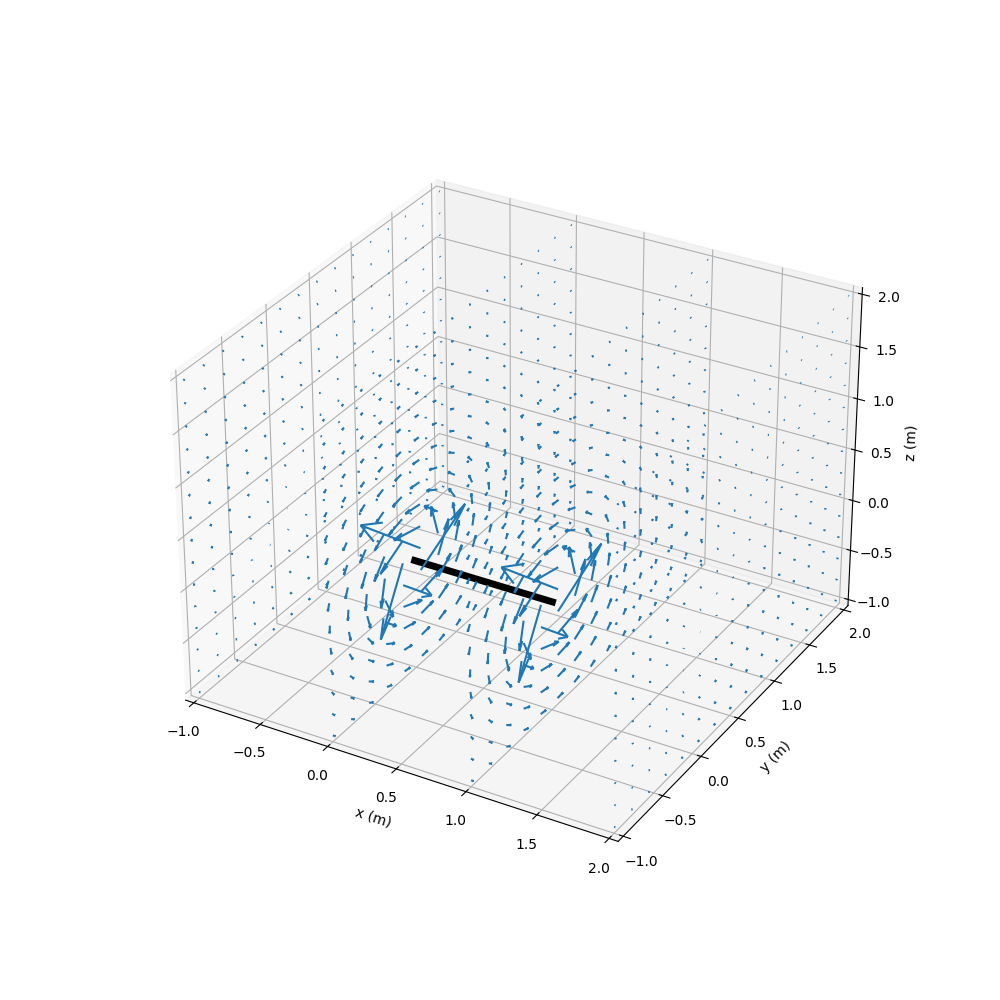
\includegraphics[width=0.8\textwidth]{/Users/lucashelal/Desktop/eel/eletromag/plots/biot_savart_1.png}
}
  Plot 2 - Normalized magnetic field in the finite wire.
{
  \centering
  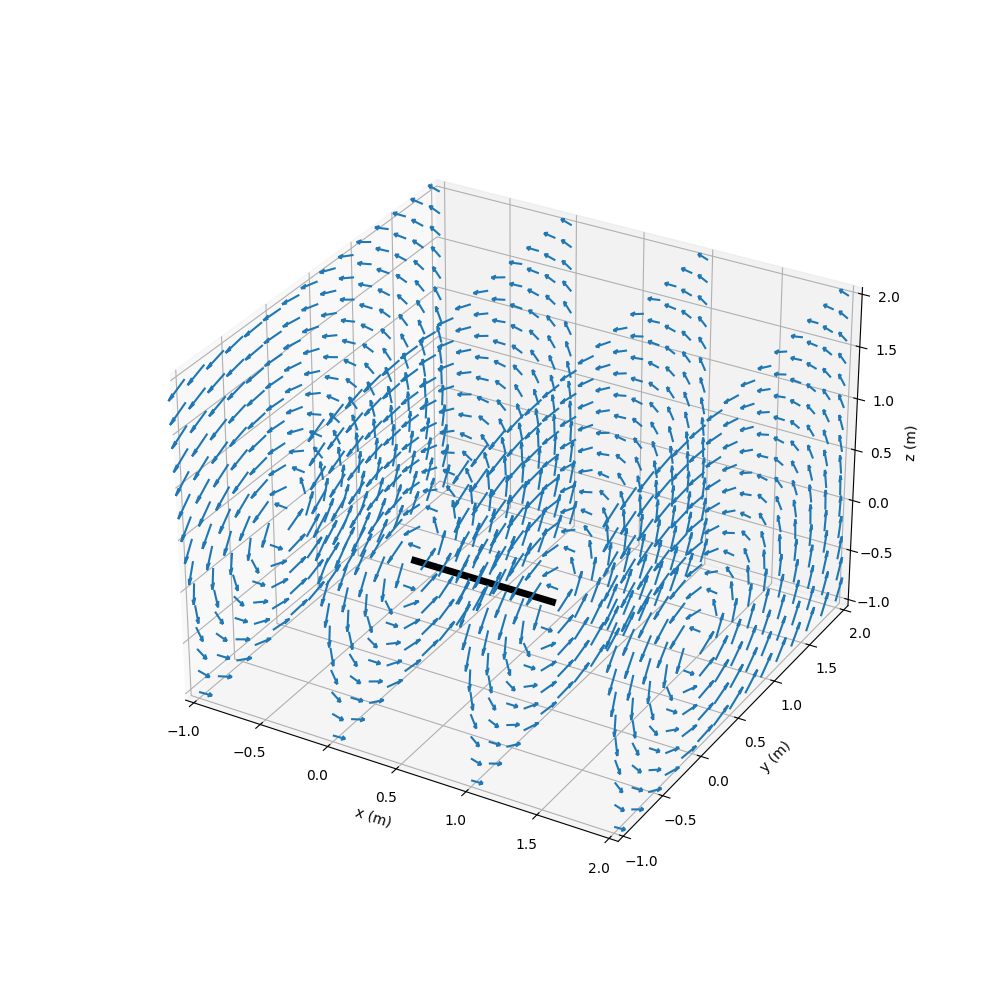
\includegraphics[width=0.8\textwidth]{/Users/lucashelal/Desktop/eel/eletromag/plots/biot_savart_normalized.png}
}
  Plot 3 - Magnetic field in the finite wire as $z_p$ component under $R^3$.
{
  \centering
  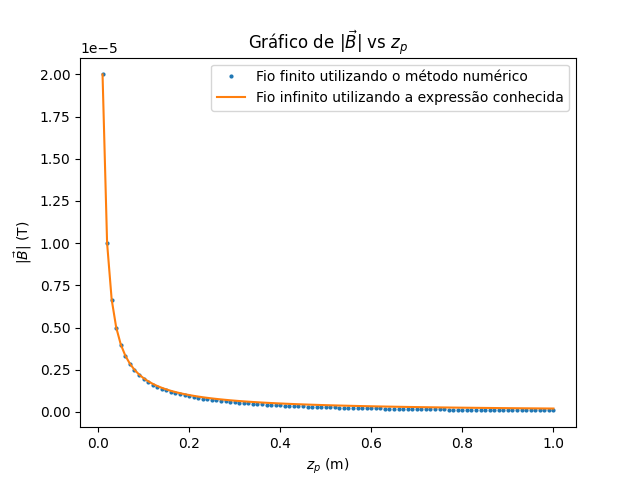
\includegraphics[width=0.8\textwidth]{/Users/lucashelal/Desktop/eel/eletromag/plots/biot_savart_zp.png}
}

\end{document}